\subsection{Generative Priors and Conditioning}
\label{sec:priors}
\subsubsection{Diffusion and Score-Based Reconstruction}
For a clean video representation $Z_0$, the standard Gaussian forward process takes the form
\begin{equation}
Z_s=\sqrt{\bar\alpha_s}Z_0+\sqrt{1-\bar\alpha_s}\,\epsilon,
\quad \epsilon\sim\mathcal N(0,I),
\end{equation}
where $s$ indexes diffusion noise rather than video time. A denoiser learns to predict noise, the clean representation, or a related velocity parameterization. Conditional restoration typically trains a denoiser using the observation representation $c(Y)$:
\begin{equation}
\mathcal L_{\epsilon}=\E\!\left[\left\|\epsilon-\epsilon_\theta(Z_s,s,c(Y))\right\|_2^2\right].
\end{equation}
DDPM, DDIM, and continuous-time score formulations provide different training and sampling perspectives~\cite{ddpm,ddim,score_sde}. Their practical role in restoration depends on what is conditioned upon, where the state lives, and whether the model was trained to describe videos or individual images.

Posterior-guided approaches instead reuse a generative prior and incorporate the observation during inference~\cite{ddrm,dps}. In latent restoration, a common approximation applies a likelihood-related gradient through a predicted clean latent and its decoder:
\begin{equation}
g_s \approx -\nabla_{Z_s}\,\ell\!\left(Y,\mathcal D_{\phi}\bigl(D(\widehat Z_0(Z_s))\bigr)\right).
\label{eq:guidance}
\end{equation}
Here $D$ is the decoder, and $\ell$ is an observation discrepancy, not necessarily an exact negative log-likelihood. The quality of this approximation depends on the noise level and the accuracy of the predicted clean representation. Unknown degradations, nonlinear codecs, errors in $\widehat Z_0$, and lossy decoding can all weaken its connection to the desired posterior. For videos, a framewise likelihood also does not automatically impose a joint temporal prior.

\subsubsection{Sources of Generative Priors}
\textbf{Training for restoration.} A task-specific diffusion process can learn a compact restoration distribution without inheriting a large text-conditioned foundation model. VD-Diff, for example, combines wavelet-aware video modeling with a learned latent prior for deblurring~\cite{vddiff}. SeedVR extends restoration-specific learning to a video transformer, while SeedVR2 combines a restoration-trained teacher with distillation and adversarial post-training~\cite{seedvr,seedvr2}. This route offers control over training data and objectives, at the cost of learning the relevant visual and motion distributions.

\textbf{Pretrained image priors.} Image diffusion models provide detailed appearance knowledge and accessible initialization~\cite{ldm}. Upscale-A-Video and StableVSR adapt image super-resolution priors with video-specific conditioning~\cite{upscale,stablevsr}. MGLD-VSR guides a latent image prior with motion information~\cite{mgld}. ZVRD and DiffIR2VR-Zero investigate transferring image priors to video without additional video-task training~\cite{zvrd,diffir2vr}. The attraction is reuse, but the missing temporal distribution must be supplied through learned modules, correspondence, sampling constraints, or a combination of these mechanisms.

\textbf{Pretrained video priors.} Video diffusion models incorporate learned spatial and temporal dependencies~\cite{svd,wan}. Their motion prior can reduce the burden on externally imposed frame coupling. Nevertheless, a model trained to generate plausible motion need not preserve the exact motion in a degraded observation. STAR uses a text-to-video foundation to support real-world VSR, DOVE adapts a video prior for efficient one-step restoration, and SVD-based methods such as DC-VSR expose the role of attention propagation across spatial and temporal partitions~\cite{star,dove,dcvsr}. The inherited motion prior reduces the amount of temporal structure that must be learned from restoration pairs, although the low-quality observation remains essential for preserving the particular motion of the input.

\textbf{Diffusion-derived representations.} A diffusion model can contribute useful representations even when the final enhancement network does not run a reverse-diffusion chain. UnDIVE transfers an encoder learned by generative pretraining into a physics-based underwater enhancement system~\cite{undive}. This use of diffusion separates representation learning from generative inference: the deployed enhancement network benefits from pretraining without executing a reverse-diffusion chain.

The amount and location of adaptation also matter when comparing pretrained video priors. LiteVSR freezes the Wan2.2-5B transformer and trains a state-aware dual-stream adapter with a lightweight fusion layer, retaining a flow-matching objective in latent space~\cite{litevsr}. Its implementation explicitly excludes pixel-domain losses, and the default evaluation uses five UniPC steps; single-step sampling is an additional supported operating point rather than the sole definition of the method. This differs from pipelines that retrain the decoder or introduce adversarial supervision after an initial latent-space stage. The division between frozen and trainable components determines both data requirements and how strongly restoration training can alter the pretrained distribution.

\subsubsection{Pixel, Feature, and Latent Representations}
Pixel-space modeling keeps the output variables close to the observation model but exposes the denoiser to the full spatial and temporal resolution. Latent diffusion reduces this cost with an encoder $E$ and decoder $D$~\cite{ldm}. Restoration then depends on both the generative model and the autoencoder's ability to preserve information. Fine text, edges, thermal structures, or small moving objects may be lost before denoising, while a framewise decoder can reintroduce flicker into a coherent latent sequence.

Spatial and temporal compression affect reconstruction in different ways. A video autoencoder with temporal compression changes the correspondence between input frames and latent tokens; treating it as a drop-in image encoder can create alignment or boundary errors. MGLD-VSR explicitly addresses temporal behavior in decoding, whereas recent efficient methods redesign or condition the decoder to reduce both cost and reconstruction loss~\cite{mgld,flash,swiftvr}. The autoencoder thus sets a representation ceiling: detail discarded during encoding or destabilized during decoding cannot be attributed solely to the denoising model.

\subsubsection{Flow Matching and Distilled Generators}
Flow matching and rectified flow learn a vector field that transports a base distribution toward a data distribution~\cite{rectifiedflow,sd3}. For a simple straight interpolation $Z_\tau=(1-\tau)\epsilon+\tau Z_0$, one illustrative objective is
\begin{equation}
\mathcal L_{\mathrm{FM}}=\E\left[\left\|v_\theta(Z_\tau,\tau,c)-(Z_0-\epsilon)\right\|_2^2\right].
\end{equation}
Inference integrates $dZ_\tau/d\tau=v_\theta(Z_\tau,\tau,c)$. This family is connected to diffusion through continuous-time generative modeling, with a distinct training path and prediction target. UniFlowRestore is an example of flow-based restoration rather than a conventional DDPM formulation~\cite{uniflowrestore}. The terminology is particularly relevant for newer video backbones and distilled restoration models.

One-step restoration may arise from teacher--student distillation, direct adaptation of a pretrained one-step model, adversarial post-training, or task-specific training. A one-step student does not retain all the iterative correction opportunities of its teacher. The training objective must absorb observation fidelity, detail generation, and temporal regularity into a single evaluation. DOVE, DLoRAL, and SeedVR2 use different routes to this goal~\cite{dove,dloral,seedvr2}; grouping them by step count alone conceals their distinct priors and training costs.

\begin{figure*}[t]
\centering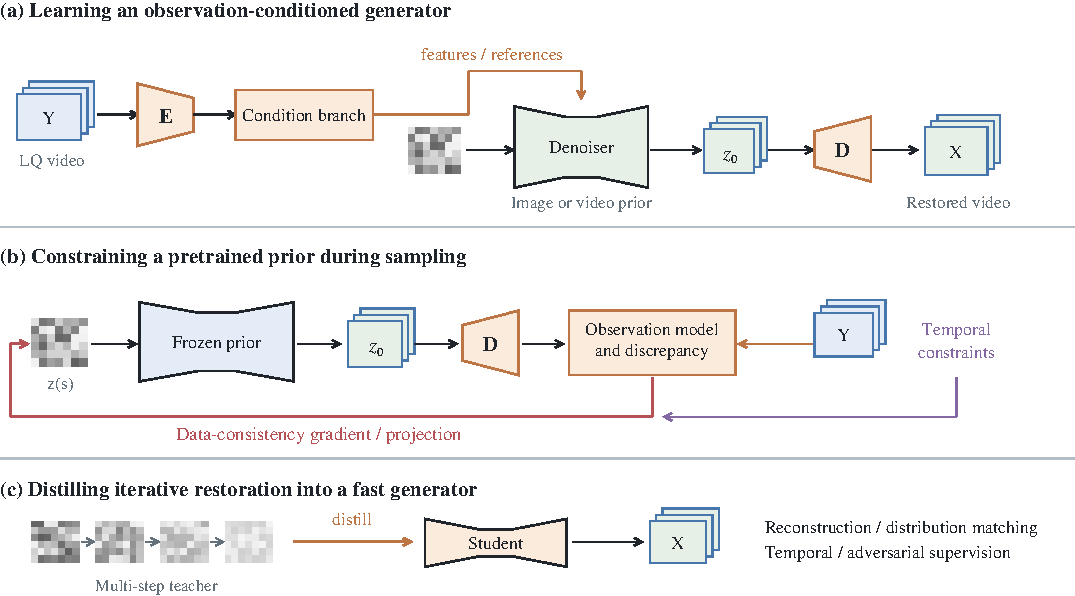
\includegraphics[width=\textwidth]{figures/prior_routes.pdf}
\caption{Three ways to connect a generative prior to video observations. (a) A learned condition branch guides denoising. (b) Observation discrepancy and temporal constraints refine sampling with a pretrained prior. (c) Distillation transfers an iterative teacher to a fast student. $E$ and $D$ denote the encoder and decoder; $Y$ and $X$ denote observed and reconstructed videos.}
\label{fig:routes}
\end{figure*}

\subsubsection{Observation and Multimodal Conditioning}
Figure~\ref{fig:routes} separates the point at which restoration evidence enters the generative process. Direct concatenation, adapters, and ControlNet-style branches feed low-quality observations into intermediate features. Observation gradients and projection-like updates act during sampling. Reference frames supply appearance or identity evidence, while optical flow, events, codec metadata, and physical image-formation models add information that an RGB-only prior may not recover reliably~\cite{cpgdnet,flair,undive,diqp}.

Text can specify a desired appearance or identify a degradation, but it usually contains less geometric evidence than the observed frames. A prompt such as ``sharp detailed face'' cannot resolve the identity of a heavily blurred person. The spatial observation therefore remains necessary even when semantic guidance improves texture generation. Similarly, strong classifier-free or task guidance can alter the balance between prior and observation, but increasing its scale is not guaranteed to improve all three quality objectives. Guidance schedules determine when semantic information shapes appearance and when observations dominate structural reconstruction.

Physical and semantic conditions can also conflict. A reference portrait may provide an identity while differing in pose, age, illumination, or expression. Codec motion vectors are useful side information but are optimized for rate--distortion coding rather than exact optical flow. Events reveal brightness changes but do not directly encode absolute radiance. Good conditioning uses each signal within its domain of validity and leaves room for uncertainty when the signals disagree.

Conditioning should be matched to the spatial and temporal support of the denoising computation. Tiled Prompts identifies a mismatch between a global caption and local latent tiles: a global description can omit a small object or impose content that is irrelevant to a particular region~\cite{tiledprompts}. It supplies local captions to image tiles or video tubes as an inference-time modification of existing super-resolution systems; the main video experiments use STAR with an I2VGen-XL backbone. Sparse visual references offer a complementary form of control. SparkVSR propagates high-resolution keyframes through a CogVideoX1.5-5B image-to-video prior while anchoring motion to the low-resolution sequence, with latent-then-pixel training and reference-free guidance~\cite{sparkvsr}. Textual and visual references thus provide different controls: local prompts constrain semantic relevance, whereas keyframes supply explicit appearance that can be propagated through the sequence.
